\chapter{\textsc{Clustering of Researchers}}
\label{chapter:clustering_of_researchers}

This chapter describes the process of clustering the \textit{Researcher-grant} and \textit{Researcher-topic} networks. The experiments are detailed, while the results are presented. Additionally, results are evaluated and discussed through comparisons to historical data and between the two \textit{Researcher} networks.

\section{Clustering of Researcher-grant network}

The process of clustering the \textit{Topic-grant} network involves a number of different stages including carrying out experiments, producing results, evaluating results as well as conducting comparative analysis.

\subsection{Experiment}

Due to the limited amount of time available and in order to ensure a consistent comparative analysis, the optimal solution identified as a result of the experiment on the \textit{Topic-grant} network, is also considered the optimal solution for the \textit{Researcher-grant} network. However, the experiment was still carried out and the results are presented in Tables 1.36-1.38, 1.43-1.45 and 1.49-1.51, part of the Supplementary material.

\subsection{Results}

The application of the optimal solution identified on the \textit{Researcher-grant} network resulted in the initial and excessive identification of 89 communities of researchers, which signifies the lack of strong and frequent collaboration relationships between researchers. Table \ref{table:researcher_b_current_numbers} presents the number of nodes representing researchers and the number and value of grants within each community discovered in the current \textit{Researcher-grant} network.

\begin{table}[!htbp]
\centering
\caption[Number of nodes and grants and value of grants within the 2 largest communities in the \textit{Researcher-grant} network constructed using the current data set (2010 to 2016)]{Number of nodes and grants and value of grants within the 2 largest communities identified in the \textit{Researcher-grant} network constructed using the current data set (2010 to 2016). The number of grants includes duplicate grants, as a grant can be part of more than one community. Subsequently, the value of grants also includes the duplicate grants. However, the last column represents the number and value of unique grants in communities within the current \textit{Researcher-grant} network.}
\label{table:researcher_b_current_numbers}
\begin{tabular}{r|rrrr}
{} & \textbf{C1} & \textbf{C2} & \textbf{Total}\\
\hline\\
\textbf{Number of researchers} & {10} & {12} & {22}\\
\textbf{Number of grants}      & {33} & {35} & {65}\\
\textbf{Value of grants} & {\pounds103M} & {\pounds87M} & {\pounds177M}\\
\end{tabular}
\end{table}

Consequently, it seems that two or more researchers collaborating multiple times as part of a grant is a rarity within the collected EPSRC data. Due to the sparse nature of the communities identified, only the two largest communities are presented in the report.

\subsubsection{Visualisation of community structure}

Similarly to the \textit{Topic-grant} network, a visualisation of the community structure discovered in the current \textit{Researcher-grant} network was produced and is presented in Fig. \ref{figure:researcher_b_current_cs}.

\begin{figure}[htpb]
    \centering
    \fbox{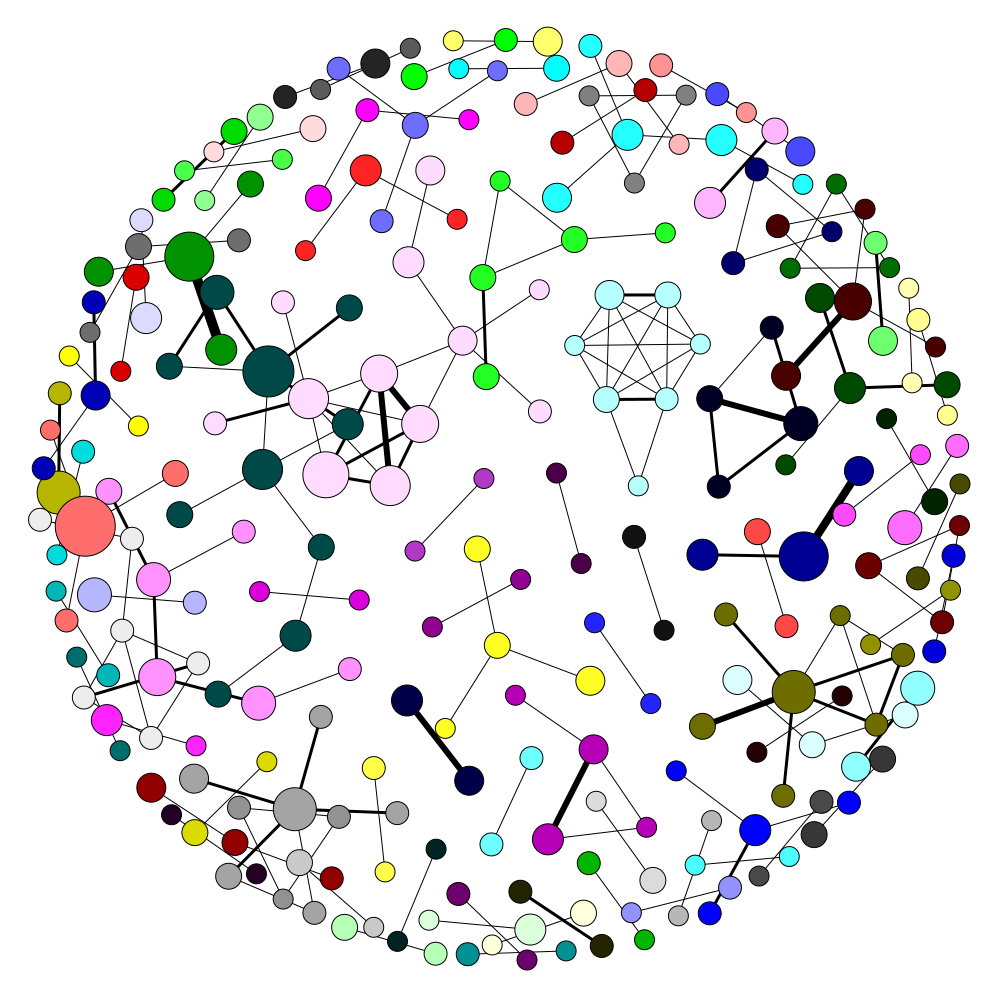
\includegraphics[width=12cm]{communities/researcher_b_cs}}
    \caption[Visualisation of the community structure within the \textit{Researcher-grant} network constructed using the current (2010 to 2016) data set]{Visualisation of the community structure within the \textit{Researcher-grant} network constructed using the current (2010 to 2016) data set.}
    \label{figure:researcher_b_current_cs}
\end{figure}

\subsection{Evaluation}

Similarly to the \textit{Topic-grant} network, the \textit{Researcher-grant} network also underwent the evaluation phase and the results show that for both the current and historical \textit{Researcher-grant} networks, nodes within the same cluster have a higher similarity than nodes from different clusters. Table \ref{table:researcher_b_evaluation} presents the results of the evaluation phase carried out on the \textit{Researcher-grant} network constructed using both the historical (1990 to 2000, 2000 to 2010) and  current (2010 to 2016) data sets.

\begin{table}[htpb]
\centering
\caption[Dice and Jaccard similarity coefficients of node pairs within and between communities in the \textit{Researcher-grant} network constructed using both the historical (1990 to 2010) and current (2010 to 2016) data sets]{Dice and Jaccard similarity coefficients of node pairs within and between communities in the \textit{Researcher-grant} network constructed using both the historical (1990 to 2010) and current (2010 to 2016) data sets. Each node pair represents an edge which connects two nodes within the same community or in two different communities. \textbf{IN} stands for within communities, while \textbf{OUT} means between communities.}
\label{table:researcher_b_evaluation}
\begin{tabular}{r|rrr}
{} & \textbf{1990-2000} & \textbf{2000-2010} & \textbf{2010-2016}\\
\hline\\
Node pairs IN                  & {1992}  & {4901}  & {206}\\
Node pairs OUT                 & {10}    & {18}    & {2}\\
Average Dice similarity IN     & {0.840} & {0.825} & {0.823}\\
Average Dice similarity OUT    & {0.342} & {0.321} & {0.336}\\
Difference between IN and OUT  & {0.481} & {0.504} & {0.505}\\
Average Jaccard similarity IN  & {0.736} & {0.740} & {0.762}\\
Average Jaccard similarity OUT & {0.210} & {0.200} & {0.202}\\
Difference between IN and OUT  & {0.526} & {0.540} & {0.560}\\
\end{tabular}
\end{table}

\subsection{Discussion}

Similarly to the \textit{Topic-grant}, the \textit{Researcher-grant} network was constructed using both the historical (1990 to 2010) and current (2010 to 2016) data sets. This means a comparative analysis can be conducted comparing the data sets in terms of research and funding trend, and clustering.

\subsubsection{Comparison to historical data}

Similarly to the historical data comparison of the \textit{Topic} networks, there is a clear funding trend which increases more rapidly the more recent the grant is. Currently, within the two largest communities, there are 65 grants worth a total value of \pounds177M. Table \ref{table:researcher_b_past1_numbers} presents the number of nodes representing researchers and the number and value of grants within each community in the \textit{Researcher-grant} network constructed using the historical (2000 to 2010) data set.

\begin{table}[!htbp]
\centering
\caption[Number of nodes and grants and value of grants within the 4 largest communities in the \textit{Researcher-grant} network constructed using the historical (2000 to 2010) data set]{Number of nodes and grants and value of grants within the 4 largest communities identified in the \textit{Researcher-grant} network constructed using the historical (2000 to 2010) data set. The number of grants includes duplicate grants, as a grant can be part of more than one community. Subsequently, the value of grants also includes the duplicate grants. However, the last column represents the number and value of unique grants in communities within the historical \textit{Researcher-grant} network.}
\label{table:researcher_b_past1_numbers}
\begin{tabular}{r|rrrrr}
{} & \textbf{C1} & \textbf{C2} & \textbf{C3} & \textbf{C4} & \textbf{Total}\\
\hline\\
\textbf{Number of researchers} & {49}  & {46}  & {55}  & {65}  & {215}\\
\textbf{Number of grants}      & {213} & {184} & {208} & {278} & {866}\\
\textbf{Value of grants}       & {\pounds87M} & {\pounds123M} & {\pounds136M} & {\pounds234M} & {\pounds551M}\\
\end{tabular}
\end{table}

From 2000 to 2010, within the four largest communities, researchers worked on 866 grants, valued at \pounds551M. These figures indicate a significant difference (798) to the number of grants completed after 2010, within the two largest communities. However, this is justified, when considering the fact that the four largest communities in the historical (2000 to 2010) data set consist of 866 grants compared to 68 grants within the two largest communities in the current (2010 to 2016) data set. More importantly, the difference in value is not significant, as the grants in the current (2010 to 2016) data set are valued higher.

Only comparing the two largest communities in both the historical (2000 to 2010) and current (2010 to 2016) data sets, the number of grants in the former is significantly larger than the one in the latter, 213 grants compared to 33 and 184 grants compared to 35. Likewise, the value of the grants is also larger, but not significantly larger, \pounds210M compared to \pounds190M. This mirrors the insights discovered during the analysis of the \textit{Topic-grant} network, as research funding increased over the years, with current grants receiving significantly more funding than grants in the past.

Furthermore, this is supported by the number and value of the grants within the five largest communities in the historical (1990 to 2000) data set. Researchers worked on a slightly less number of grants than between 2000 and 2010, but they also received significantly less funding, \pounds130M in total. Table \ref{table:researcher_b_past2_numbers} presents the number of nodes representing researchers and the number and value of grants within each community in the \textit{Researcher-grant} network constructed using the historical data set (1990 to 2000).

\begin{table}[!htbp]
\centering
\caption[Number of nodes and grants and value of grants within the 5 largest communities in the \textit{Researcher-grant} network constructed using the historical (1990 to 2000) data set]{Number of nodes and grants and value of grants within the 5 largest communities identified in the \textit{Researcher-grant} network constructed using the historical (1990 to 2000) data set. The number of grants includes duplicate grants, as a grant can be part of more than one community. Subsequently, the value of grants also includes the duplicate grants. However, the last column represents the number and value of unique grants in communities within the historical \textit{Researcher-grant} network.}
\label{table:researcher_b_past2_numbers}
\begin{tabular}{r|rrrrrr}
{} & \textbf{C1} & \textbf{C2} & \textbf{C3} & \textbf{C4} & \textbf{C5} & \textbf{Total}\\
\hline\\
\textbf{Number of researchers} & {31}  & {21} & {46}  & {35}  & {30}  & {163}\\
\textbf{Number of grants}      & {115} & {78} & {150} & {147} & {129} & {610}\\
\textbf{Value of grants} & {\pounds34M} & {\pounds18M} & {\pounds21M} & {\pounds41M} & {\pounds17M} & {\pounds130M}
\end{tabular}
\end{table}

\subsubsection{Motivation the Researcher-topic network}

Similarly to the \textit{Topic-researcher} network, the \textit{Researcher-topic} network represents an alternative to the \textit{Researcher-grant} network. Therefore, both Researcher networks are considered important due to the different and valuable insights that can be translated from the data.

\clearpage

\section{Clustering of Researcher-topic network}

The process of clustering the \textit{Researcher-topic} network involves a number of different stages including carrying out experiments, producing results, evaluating results as well as conducting comparative analysis.

\subsection{Experiment}

Due to the limited amount of time available and in order to ensure a consistent comparative analysis, the optimal solution identified as a result of the experiment on the \textit{Topic-grant} network, is also considered the optimal solution for the \textit{Researcher-topic} network. However, the experiment was still carried out and the results are presented in Tables 1.55-1.57, part of Supplementary material.

\subsection{Results}

In contrast to the \textit{Researcher-grant} network, the application of the optimal solution identified on the \textit{Researcher-topic} network resulted in the less excessive initial identification of 49 communities of researchers. However, the number of identified communities is still too large and represents communities consisting of small numbers of researchers that have a small number of topics in common.

Furthermore, it seems that a large number of researchers having multiple common topics is a rarity within the EPSRC data. Due to the sparse nature of the communities identified, the eight largest communities are presented here. Table \ref{table:researcher_a_current_numbers} presents the number of nodes representing researchers within the eight largest communities in the \textit{Researcher-topic} network.

\begin{table}[!htbp]
\centering
\caption[Number of nodes within the eight largest communities in the \textit{Researcher-topic} network constructed using the current data set (2010 to 2016)]{Number of nodes within the eight largest communities identified in the \textit{Researcher-topic} constructed using the current (2010 to 2016) data set.}
\label{table:researcher_a_current_numbers}
\begin{tabular}{r|rrrrrrrrr}
{} & \textbf{C1} & \textbf{C2} & \textbf{C3} & \textbf{C4} & \textbf{C5} & \textbf{C6} & \textbf{C7} & \textbf{C8} & \textbf{Total}\\
\hline\\
\textbf{Number of researchers} & {60} & {120} & {30} & {24} & {43} & {48} & {126} & {46} & {225}
\end{tabular}
\end{table}

\subsubsection{Visualisation of community structure}

Similarly to the \textit{Topic-grant} network, a visualisation of the community structure discovered in the current \textit{Researcher-topic} network was produced and is presented in Fig. \ref{figure:researcher_b_current_cs}.

\begin{figure}[!htpb]
    \centering
    \fbox{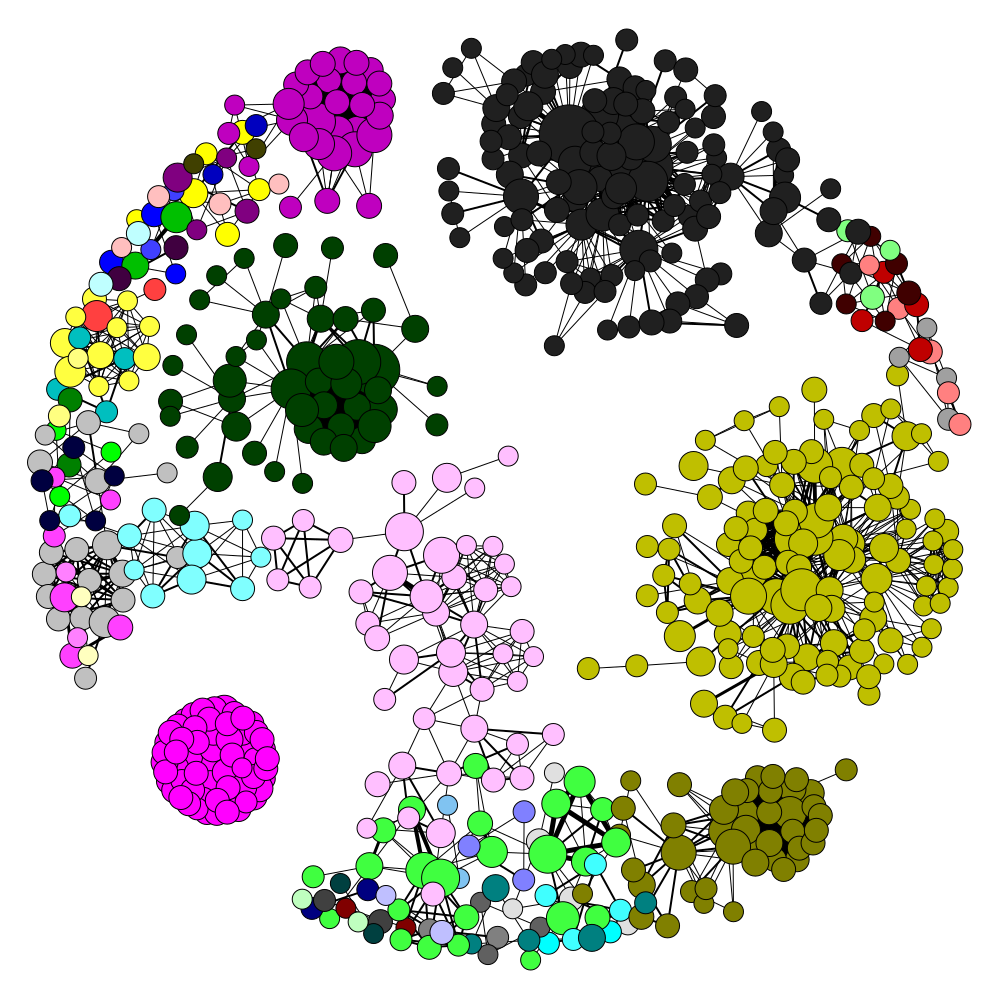
\includegraphics[width=13cm]{communities/researcher_a_cs}}
    \caption[Visualisation of the community structure within the \textit{Researcher-topic} network]{Visualisation of the community structure within the \textit{Researcher-topic} network constructed using the current (2010 to 2016) data set.}
    \label{fig:researcher_a_current_cs}
\end{figure}

\subsection{Evaluation}

Similarly to the \textit{Topic-grant} network, the \textit{Researcher-topic} network also underwent the evaluation phase and the results show that nodes within the same cluster have a higher similarity than nodes from different clusters. Table \ref{table:researcher_a_evaluation} presents the results of the evaluation phase carried out on the \textit{Researcher-topic} network constructed using the current (2010 to 2016) data set.

\begin{table}[htpb]
\centering
\caption[Dice and Jaccard similarity coefficients of node pairs within and between communities in the \textit{Researcher-topic} network constructed using the current (2010 to 2016) data set]{Dice and Jaccard similarity coefficients of node pairs within and between communities in the \textit{Researcher-topic} network constructed using the current (2010 to 2016) data set. Each node pair represents an edge which connects two nodes within the same community or in two different communities. \textit{IN} stands for within communities, while \textit{OUT} means between communities.}
\label{table:researcher_a_evaluation}
\begin{tabular}{r|r}
{} & \textbf{2010-2016}\\
\hline\\
Node pairs IN                  & {4273}\\
Node pairs OUT                 & {275}\\
Average Dice similarity IN     & {0.835}\\
Average Dice similarity OUT    & {0.405}\\
Difference between IN and OUT  & {0.430}\\
Average Jaccard similarity IN  & {0.779}\\
Average Jaccard similarity OUT & {0.273}\\
Difference between IN and OUT  & {0.506}\\
\end{tabular}
\end{table}

\subsection{Discussion}

The \textit{Researcher-grant} and \textit{Researcher-topic} networks represent two interpretations of the researcher data. This means a comparative analysis can be conducted comparing the two networks in terms of clustering.

\subsubsection{Comparison to Researcher-topic network}

The clustering results produced using both networks clearly indicate that the \textit{Researcher-topic}  network is the more rational and valuable interpretation of the researcher data, as expected prior to the creation process of the \textit{Researcher} networks.

In one hand, there is a network that consists of researchers and links between them symbolising a work collaboration between the two. As proved by the results, this is fairly rare in the academic world. Unless two researchers have a relationship, are part of the same institution or organisation or are located in the same city, it is hard to believe that they would collaborate on multiple occasions. Moreover, it is essential to note that there is a clear difference between collaborating on a government-funded grant and any other research project. Certain grants can last up to 7 years and at the end of the grant the researchers that worked on it will most probably not collaborative again for a lengthy period of time, if at all. In conclusion, the grant-based interpretation of the researcher data did not prove to be significantly valuable. However it did provide interesting insights into the progress of research and research funding over a 26-year long period.

On the other hand, there is a network that consists of researchers and links between them symbolising a shared research interest between the two. This type of connection between two researchers is not limited to a relationship, institution or organisation, or location. Only a shared research interest is required. In the academic world, this is very common as researchers from all over the world can connect and relate to each other through a common research field. The ideal result from such a network is a fairly low number of communities consisting of researchers that share an interest in a number of different topics. However, due to the large number of researchers, the number of identified communities turns out to be large and at the same time, sparse. That being said, this interpretation of the data is still a better option than the first, as it produces a more compelling clustering based on the researcher data available.